\noindent While most methods are detailed in the papers presented in the following chapters, these sections aim to fill certain gaps and delve into the developed algorithms included in DeepOF that were not applied in the results presented in chapter \ref{chap:natcomm}.
 
\section{Software architecture and deployment}

The software package presented in this thesis, called DeepOF, was developed using a modular approach consisting of three primary modules designed for user interaction (called \python{deepof.data}, \python{deepof.post\_hoc}, and \python{deepof.visuals}), and five modules for internal calculations. A comprehensive list and description of all modules follows:

\begin{itemize}
    \item \texttt{deepof.data} - Includes tools for data loading, preprocessing, and pattern extraction
    \item \texttt{deepof.post\_hoc} - Includes tools for post-hoc analysis tools for results obtained with annotation pipelines
    \item \texttt{deepof.visuals} - Includes a comprehensive set of visualization functions
    \item \texttt{deepof.utils} - Includes general utilities
    \item \texttt{deepof.models} - Contains code for the deep clustering model architectures
    \item \texttt{deepof.hypermodels} - Contains hypermodels for hyperparameter tuning of the deep clustering models
    \item \texttt{deepof.annotation\_utils} - Contains utilities for the supervised annotation pipe\-line
    \item \texttt{deepof.model\_utils} - Contains utilities for the unsupervised pipeline (including model training and evaluation)
\end{itemize}


Furthermore, DeepOF also features a suite of automated tests with continuous integration (CI) to ensure the proper functioning of all deployed code. These were implemented using the hypothesis package for Python, a suite that enables property-based testing, where synthetic examples are created on the fly to test all functions while following a set of defined constraints \cite{Maciver2019Hypothesis:Testing}. Test coverage is reported automatically, and computed using the \python{coverage} package for Python \cite{Coverage.pyDocumentation}. 

Documentation was written and deployed using read-the-docs \cite{HomeDocs}, and automatic API pages were created using \python{autodoc}. Contributing guidelines and a code of conduct are also included.

\section{Data loading and input}

DeepOF takes a set of two files per experiment that was carried out, including a video (various standard formats are accepted) and a table containing the tracking output generated with DeepLabCut (which can be in either CSV or HDF). Upon importing the package, the project is initialized as an instance of the \python{Project} class available in \python{deepof.data}, and excecuted using the \python{.create()} method, which applies all parameters and processing and stores the results in an instance of the \python{Coordinates} class, also in \python{deepof.data}. From here, many sets of features can be extracted as instances of the \python{TableDict} class (also in \python{deepof.data}), and the supervised and unsupervised annotation pipelines can be excecuted (see \href{https://deepof.readthedocs.io/en/latest/}{full documentation} for more details).

\section{Time series processing}

All relevant details on time series processing \fullncref. 

\section{Supervised annotation of pre-defined traits}

All relevant details on the supervised annotation of pre-defined traits \fullncref. 

\section{Unsupervised annotation: exploring the behavioral space}

As previously mentioned, DeepOF includes a pipeline for motion tracking time series segmentation, which retrieves behaviors that are expressed consistently throughout the filmed animal experiments. This pipeline provides a series of architectures and data input objects to choose from according to the nature of the captured video. To start with, let us explore how the input for time series segmentation can be represented. 

\subsection{Matrix input/output representations}

The simplest way to arrange time series as input for the unsupervised pipeline is the same used by the models from the literature presented in \cref{chap:sota}. That is, as matrices of features over time, where different attributes are assumed to be independent. Moreover, sliding windows are cross-correlated with these time series, to end with a three-dimensional tensor representation where dimensions correspond to sliding window instances, time within each window, and features, respectively (Figure~\ref{fig:3.1}, left).

\subsection{Graph input/output representations}

While sufficient in many cases (as in the packages mentioned in \cref{chap:sota}, where paws are accessible when experimenters are filming from below), matrix representations assume that features are spatially independent, which is not the case.
To examine the possibility of including spatio-temporal relationships between the features, we included in DeepOF the option to represent tracking data as dynamic graphs (Figure~\ref{fig:3.1}, right). While connectivity in these graphs (whose adjacency matrix links body parts that are spatially adjacent) remains static, features are organized as node and edge attributes that vary across time. Moreover, this enables the program to incorporate more features naturally: this way, not only coordinates but also velocities are included as node attributes, and distances between pairs of body parts are used to annotate edges.
Furthermore, this representation can be expanded to accommodate multiple animals, where separate graph representations for each animal are connected via nose-to-nose, nose-to-tail, and tail-to-tail edges, enabling the models to include relative distances between animals. When this is the case, an $L_1$ penalization over the node embeddings controls the influence social interactions should have in the results, over the posture of individual animals. When using graph representations, inputs to the segmentation models are three fold, and include:

\begin{itemize}
    \item A four dimensional tensor with \textbf{node attributes}, with dimensions corresponding to sliding window instances, time within each window, nodes in the graph, and features in each node.
    \item A four dimensional tensor with \textbf{edge attributes}, with dimensions corresponding to sliding window instances, time within each window, edges in the graph, and features in each node.
    \item the \textbf{adjacency matrix} of the graph to embed, which remains static throughout time.
\end{itemize}

\begin{figure}[!thb]
\centering
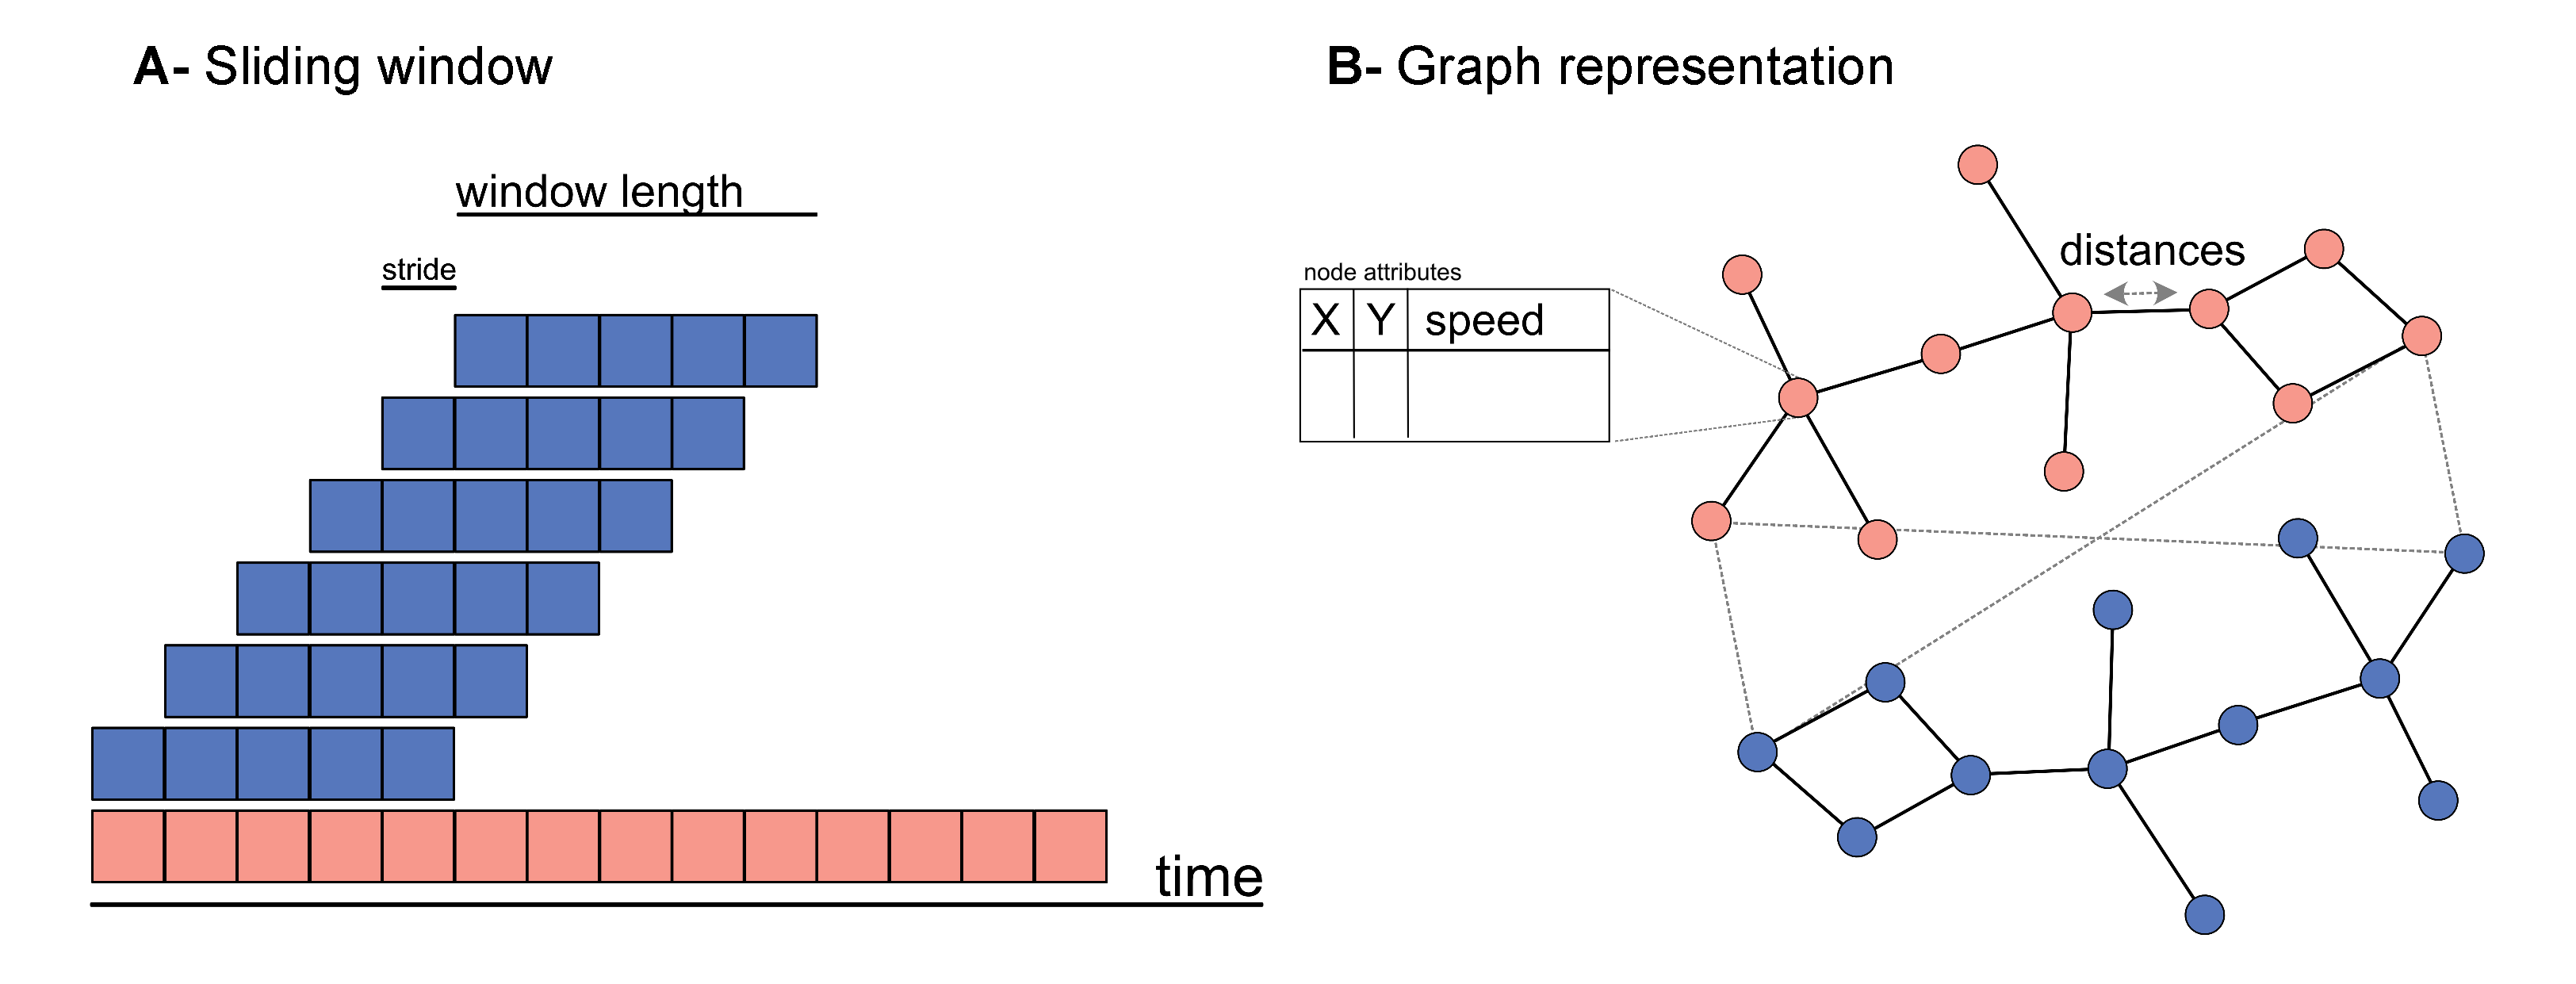
\includegraphics[width=\textwidth]{Figures/methods_1.pdf}

\caption[\textbf{Time series input representation for deep clustering of motion tracking data}]{\textbf{Time series input representation for deep clustering of motion tracking data:} \textbf{A}: Prior to segmentation model training, time series are split using a sliding window approach. The length and stride of the windows are hyperparameters that the user can modify, and default to the frame rate of the videos (so that each window includes one second of motion data) and one, respectively. \textbf{B}: To leverage spatial correlations between the features, and allow for the natural inclusion of features other than coordinates, input time series can be represented as dynamic graphs. Here, connectivity remains static, while node and edge attributes vary through time. Moreover, this representation paves the way to include multiple animals in a single model, since edges between body parts of different animals can be incorporated.}
\label{fig:3.1}

\end{figure}

\section{Unsupervised annotation: deep clustering models}

As part of the first goal of this thesis, as defined in the last section of \cref{chap:sota}, DeepOF includes three families of deep representation models for time series segmentation. Each of these families (described in the following sections) can be used with matrix or graph input representations. Moreover, their encoder (and decoder, when applicable) structures can be selected from a set of recurrent, TCN, and transformer-based architectures. 

\begin{figure}[!thb]
\centering
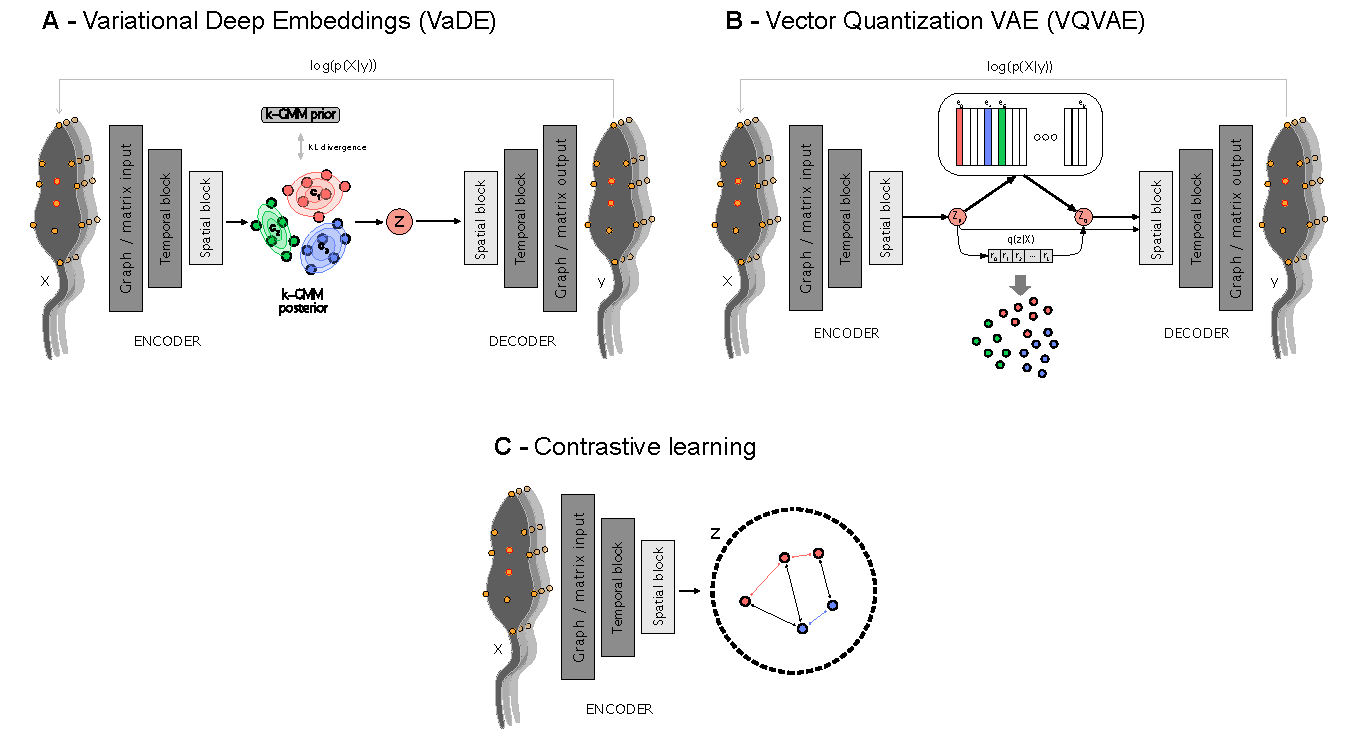
\includegraphics[width=\textwidth]{Figures/methods_2.pdf}

\caption[\textbf{Deep clustering architectures implemented within DeepOF}]{\textbf{Deep clustering architectures implemented within DeepOF:} \textbf{A}: Variational Deep Embeddings (VaDE): the model follows an encoder-decoder architecture similar to a variational autoencoder, with the key difference that both latent space and prior distribution are mixtures of multivariate Gaussians instead of unimodal distributions. This not only imposes a clustering structure in the latent space $Z$, but also allows to directly extract soft cluster assignments at inference time, as the normalized likelihood under each component of the mixture. \textbf{B}: Vector-Quantization Variational Autoencoders (VQVAE): similar to VaDE, the model follows an autoencoder-like architecture. Instead of having a probability distribution as a prior, there is a discrete codebook being maintained in parallel to the model, whose columns represent cluster centroids on the latent space. At training time, the closest entry in the codebook to the current embedding vector is selected and passed through the decoder instead of the vector itself. The model is trained to reconstruct the input and to minimize the Euclidean distance between each latent vector $z$ and its closest codebook entry. At prediction time, clusters are assigned to the closest codebook entry for the embedding obtained for each input instance. \textbf{C}: Contrastive learning: this architecture consists only of an encoder that maps each input instance to a latent space $Z$. A contrastive loss pulls together similar embeddings (represented with colored arrows between points of the same color, and pushes apart dissimilar embeddings (represented with black arrows between points of different colors). The definition of what \textit{similar} and \textit{dissimilar} mean in this context depends on the loss function of choice. This is the only provided architecture that requires post-hoc clustering of the latent space.}
\label{fig:3.2}

\end{figure}

When a graph representation is selected as input, these temporal blocks are coupled with graph neural network (GNN) spatial blocks capable of embedding both node and edge attributes \cite{Jiang2020Co-embeddingNetworks}, building what is known as spatio-temporal graph neural network (ST-GNN) structures \cite{Li2021MultiscalePrediction, Sahili2023Spatio-TemporalSurvey}. This gives DeepOF flexibility to adapt to different data scenarios and hardware systems, as will be discussed in chapter~\ref{chap:discussion}. The next few sections introduce the three families of deep representation models included in DeepOF, which are based in Variational Deep Embeddings (VaDE), Vector Quantization Variational Autoencoders (VQVAE), and self-supervised contrastive learning architectures, respectively. Schematic representations of all three can be found in Figure~\ref{fig:3.2}.

\subsection{Variational Deep Embeddings (VaDE)}

The first segmentation architecture available in DeepOF is based on Variational Deep Embeddings (VaDE) \cite{Jiang2016VariationalClustering, Manduchi2021AData}, a deep clustering algorithm that consists of an encoder-decoder architecture similar to that of a Variational Autoencoder (VAE) \cite{Kingma2013Auto-EncodingBayes}. Here, an encoder neural network maps the input $X$ to a latent vector $z$, and a decoder architecture maps such vector to the output $y$. As the traditional VAE, the model is trained to minimize the evidence lower bound (ELBO) which is a composite loss function that aims to minimize both the reconstruction error given the input, and the Kullback-Leibler (KL) divergence between the latent vectors and a prior distribution. Unlike the traditional VAE, however, VaDE architectures map the input vectors to a mixture of (in this case Gaussian) distributions, with each component representing a given cluster. Formally, the training process aims to minimize the equation:

\begin{equation}
L_\mathrm{ELBO}(x) = \mathbb{E}_{q(z,c|x)}[\log p(x|z)] - D_\mathrm{KL}(q(z,c|x) || p(z,c))
\label{eq:3.1}
\end{equation}

\noindent where the first term corresponds to the reconstruction loss, which encourages the latent space ($z$) to represent the data ($x$) well over a set of clusters ($c$). The second term is the aforementioned KL divergence ($D_\mathrm{KL}$) between a Gaussian mixture prior ($p(z,c)$) and the variational posterior for each cluster ($q(z,c|x)$). This serves the purpose of regularizing the embeddings to also follow a Gaussian mixture distribution, where each component is associated with a particular cluster. A schematic overview of the model can be found in Figure~\ref{fig:3.2}A.
Importantly, this loss function imposes a clustering structure directly within the latent space, eliminating the need for post-hoc clustering of embeddings required by other existing tools. This end-to-end approach offers several benefits, with the primary advantage being that the clustering structure back-propagates to the encoder during training.

After the models are trained, cluster assignments are obtained as the \python{argmax} of the posterior distribution given the data, as outlined in equation~\ref{eq:3.2}:

\begin{equation}
q(c|x) = p(c|z) \equiv \frac{p(z)p(z|c)}{\sum_{c'=1}^K p(c')p(z|c')}
\label{eq:3.2}
\end{equation}

\noindent where $c'\in(1, K)$ is an iterator over all clusters in the model.
In practice, this unsupervised pipeline can retrieve consistent patterns of animal motion in a flexible, non-linear, and fully unsupervised way. Moreover, training is stable for all encoder-decoder architectures and input structures included in the package. This makes it the ideal default for the unsupervised segmentation pipelines. All results presented in \cref{chap:natcomm} use this architecture.

\subsection{Vector Quantization Variational Autoencoders (VQVAE)}

The second implemented segmentation model to visit is an adapted version of the vector quantization variational autoencoder architecture (VQVAE) \cite{VanDenOord2017NeuralLearning}. This also follows an encoder-decoder architecture, minimizes the mean squared error reconstruction loss between input and output, and enforces a clustering structure in the latent space in an end-to-end fashion. The main difference with VaDE is that this clustering structure is approached using vector quantization, which enforces a discrete latent space instead of a continuous probability distribution \cite{VanDenOord2017NeuralLearning}. In practice, the input $X$ is passed through a sequence-aware encoder onto an embedding vector $z_p$, which is compared to the columns of a separately maintained codebook (represented as a matrix whose column vectors are cluster centroids). The closest codebook column vector ($z_q$) is then selected (Eq.~\ref{eq:3.3-3.4}) and passed on to the decoder instead of $z_p$ itself:

\begin{align}
q(z = k|x) &= \begin{cases}
    1 & \text{for } k = \mathrm{argmin}_j\|z_p(x) - e_j\|_2, \\
    0 & \text{otherwise}.
\end{cases} \\
z_q(x) &= e_k, \text{ where } k = \mathrm{argmin}_j\|z_p(x) - e_j\|_2
\label{eq:3.3-3.4}
\end{align} 

\noindent where $e_j$ is a given column of the codebook. The model is then trained to maximize the conditional log-likelihood of the data, $\log(p(X|z_q(x))$, and minimize the Euclidean distance between $z_p$ and $z_q$ (often referred to as \textit{commitment loss}).

Moreover, a key aspect of the VQVAE setting is that the described lookup operation is non-differentiable, which prevents gradients from flowing through the encoder during backpropagation, preventing proper training. In the original paper, this problem is overcome by copying the gradients through the lookup (from $z_p$ to $z_q$). Later work, however, suggested that while such an approximation works well in the image compression setting originally presented, it is not ideal for clustering since the required number of codes is much smaller, which increases the average distance between $z_p$ and $z_q$ during training, making the gradients less informative and leading to a suboptimal encoder \cite{Fortuin2018SOM-VAE:Series}. To mitigate this issue, we followed existing approaches and added a second reconstruction loss, which connects $z_p$ with the decoder, bypassing the lookup operation and enabling gradient flow. A scheduler decreases the weight ($\alpha$) of the loss assigned to this term as training progresses, once the average distances between $z_p$ and $z_q$ are close. The complete loss function is thus defined as:

\begin{equation}
L = \log p(x|z_q(x)) + \alpha \log p(x|z_p(x)) + \beta \left\|z_p(x) - z_q(x)\right\|_2^2
\label{eq:3.5}
\end{equation}

Once the models are trained, cluster assignments can be obtained using the same lookup operation described in equation \ref{eq:3.3-3.4}. Moreover, soft counts can be obtained using the fuzzy-c means approach, where confidence is inversely proportional to the distance to the closest centroid \cite{Bezdek1984FCM:Algorithm}.

In practice, this model is faster to train than VaDE when all other parameters are left equal, and it is still end-to-end. While this may make it preferable in some hardware-constrained situations, training was shown to be unstable when coupled with graph inputs, making it a poorer overall default choice, especially in top-down video settings. All results presented in the original DeepOF preprint \cite{Bordes2023AutomaticallyStress}, posted in bioRxiv, make use of this architecture.

\subsection{Contrastive representation learning (CRL)}

A third representation and segmentation pipeline is included in DeepOF as an option that, although not end-to-end, I believe deserves to be mentioned. Contrastive learning is a set of representation learning approaches that fall into what the literature has called \textit{self-supervised learning}. In contrast to the two models presented above, which are generative approaches to representation learning (since they directly model the data distribution, and their decoders can explicitly be used to generate data), \textit{self-supervised} approaches use discriminative models instead. This eliminates the need for a potentially wasteful decoder, making learning more efficient when representations are the only goal \cite{Le-Khac2020ContrastiveReview}. 

Contrastive representation learning in particular works by applying a loss function directly to the latent space, and following a simple principle: \textit{similar} samples (denoted as \textbf{positive pairs}) should be pulled together, whereas \textit{dissimilar} samples (\textbf{negative pairs}) should be pulled apart. The trick lies in defining what similarity means in this case: given a sample, these approaches sample a positive pair from a positive distribution ($x^{+} \sim p^{+}(\, \cdot\, | x)$), and a negative pair from a negative distribution ($x^{-} \sim p^{-}( \,\cdot\, | x)$). In DeepOF, positive and negative sampling are based on recently introduced time-series change-point detection contrastive models \cite{Deldari2021TimeCoding}, where samples closer in time have a higher probability of being called a positive pair, and vice versa. Once positive and negative pairs are defined, the default algorithm applies the \textit{InfoNCE} (Noise Contrastive Estimation) loss \cite{vandenOordDeepMind2019RepresentationCoding}, which maximizes the mutual information between consecutive time windows. Thus, a single positive pair of time adjacent intervals ($h_i, f_i$, where $h_i$ is called the history window, and $f_i$ the future window), and a set of $K - 1$ negative pairs where the intervals $h_i$ and $f_j$ are well separated in time across the sequence, can be used to calculate the normalized similarity $\rho_i$ across all pairs:

\begin{equation}
\rho_{i} = \frac{\exp(\Sim(h_{i}, f_{i})/\tau)}{\sum_{j=1}^{K}\exp(\Sim(h_{i}, f_{j})/\tau)}
\label{eq:3.6}
\end{equation}

\noindent where $\tau$ is a scaling parameter and $\Sim$ is the cosine similarity between each pair of data embeddings \cite{Deldari2021TimeCoding}. The final loss is then computed by applying the binary cross-entropy function over the similarities of all pairs:

\begin{equation}
\mathcal{L} = -\sum_{i,j} y_{ij} \log(\rho_{i}) + (1 - y_{ij}) \log(1 - \rho_{i})
\label{eq:3.7}
\end{equation}

This model has several advantages over the previous two when it comes to learning representations. For starters, it has substantially fewer parameters since it lacks a decoder, which can make training substantially faster. Moreover, the success of contrastive representation learning so far has been linked to improved abstraction (the extraction of concepts that are invariant to local or small changes in the data) and disentanglement (with uncorrelated latent dimensions representing qualitatively different concepts) of representations in many scenarios \cite{Le-Khac2020ContrastiveReview}. However, no noticeable improvements in this regard were obtained so far in DeepOF. Moreover, and as mentioned at the beginning of this section, the provided contrastive models do not enable end-to-end clustering, with cluster assignments needing to be obtained in a post-hoc fashion. DeepOF does this by fitting a Gaussian HMM to the trained latent space \cite{Schreiber2017Pomegranate:Python}. While it does not escape my attention that HMM parameters could be learned jointly with the neural network in theory, thus making the model truly end-to-end, all attempts so far resulted in unstable training. Further efforts in this direction for future releases of the package are not discarded.

\subsection{Semi-supervised post-hoc reclustering}

While both VaDE and VQVAE models offer end-to-end clustering, they do so by grouping similar sliding window instances on a shuffled dataset, without a clear explicit idea of how the sliding windows are ordered across time. While significantly overlapping windows mitigate this issue, in practice there are sections in the experiments where low-confidence cluster assignments often switch between states, requiring the user to discard them for further analysis. To avoid this problem altogether, DeepOF can train a semi-supervised HMM to the latent space \cite{Schreiber2017Pomegranate:Python}, where prior probabilities are assigned to each sample as the VaDE / VQVAE soft counts, and posteriors are obtained by fitting a Gaussian HMM. The overall effect leads to cleaner cluster assignments across time, and longer average times on each cluster.

\section{Characterization of Chronic Social Defeat Stress (CSDS)}

Details on animal handling, CSDS protocols, behavioral testing, datasets used, and experimental design \fullncref. 

\section{DeepOF in practice and post-hoc analysis of annotation results}

All relevant details on the post-hoc analysis of both supervised and unsupervised annotation results \fullncref.

\section{Statistics}

Statistical analyses and graphs were made in R (v 4.1.1), python (v 3.9.13), and DeepOF (v0.4.6). Details on tests and assumptions when comparing samples, as well as multiple testing corrections and notation, \fullncref.